\documentclass{article}
\usepackage{ctex}
\usepackage{graphicx}
\usepackage{amsmath}
\usepackage{indentfirst}
\usepackage{titlesec}
\usepackage{setspace}
\usepackage{subfigure}
\usepackage{caption}
\usepackage{float}
\usepackage{booktabs}
\usepackage{geometry}
\usepackage{multirow}
\geometry{left=1.2cm,right=1.2cm,top=2cm,bottom=2cm}
\title{\songti \zihao{2}\bfseries 柱矢量光束的产生与检测预习报告}
\titleformat*{\section}{\songti\zihao{4}\bfseries}
\titleformat*{\subsection}{\songti\zihao{5}\bfseries}
\renewcommand\thesection{\arabic{section}}
\author{王启骅 PB20020580}
\begin{document}
	\maketitle
	\section{实验目的}
	柱矢量光束(包括径向偏振光和角向偏振光)电场振动方向在光束横截面上具有轴对称性,光束的波振面呈漩涡状,且中心
	呈现奇异性。柱矢量光束主要包括径向偏振光和角向偏振光,径向偏振光的偏振方向呈辐射状分布,角向偏振光为环绕状分布。相对于传统单一偏振态分布的光束,柱矢量偏振光束呈现出很多不同的性质,其中最重
	要的特点是经过高数值孔径透镜聚焦后的场强分布。柱矢量偏振光束产生方法主要包括主动式和被动式两类,主动式为激光腔内谐振输出的
	光束即为所述光束,被动式指的是既有的普通激光光束通过一些转化装置变为柱矢量光束。
	
	本实验以被动方式,探究柱矢量光的产生并检验。
	\section{实验原理}
	一束线偏振光经过一个$ \frac{\lambda}{2} $ 波片,偏振方向与波片的慢轴夹角为$\theta$,透射后其偏振方向发
	生变化。入射光的快轴分量经过片相对提前了,出射光的偏振方向与慢轴夹角为
	-$\theta$。根据上述分析,就可以很好的理解本实验中所用的拼接半波片方法产生柱矢量偏振光束
	的原理。(相当于以慢轴镜面反射)
	
	
	一块 8 片拼接波片装置,相邻的波片之间的慢轴夹角为 22.5°,
	一束如图线偏光通过它之后变为径向偏振光。
	\begin{figure}[!h]
		
		\centering
		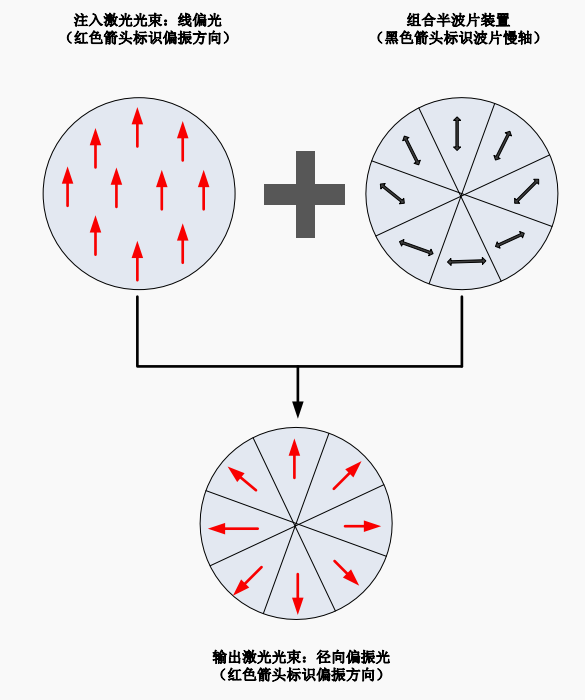
\includegraphics[scale=0.56]{a}
		\captionsetup{font={small},labelfont=bf}
		\caption{\heiti\zihao{-5}波片及效果}
		
	\end{figure}


\section{实验装置}

如图2为实验光路装置
	\begin{figure}[!h]
	
	\centering
	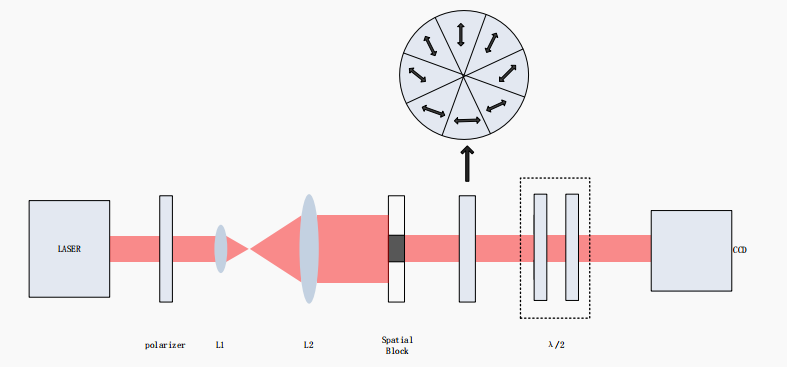
\includegraphics[scale=0.7]{光路图}
	\captionsetup{font={small},labelfont=bf}
	\caption{\heiti\zihao{-5}实验光路图}
	
\end{figure}


激光器出射光束经过偏振片后变为线偏光,一般激光机器出射光束的偏振特性都比
较好,经过两个焦距不同的共焦透镜将光束放大并准直,再经过光阑选择均匀的圆形平行光束
圆形光束中心经过拼接半波片装置中心奇点,产生中心偏振奇点的柱矢量光束。
虚线框内的两个级联片可以将径向偏振光变为角向偏振光;之后通过倒置的透镜
组后用 ccd 接收并观测。

\section{实验步骤}
1 调整光路,在未加级联片的情况下,使之输出径向偏振光束,并且利用偏振片检查其偏振
特性,记录实验图像。


2 加入级联片,调节输出角向偏振光束,并且利用偏振片检查其偏振特性,记录实验图像。


3 在不使用级联片的情况下,利用一块波片使之输出角向偏振光。

\end{document}